\documentclass{article}\usepackage[]{graphicx}\usepackage[]{xcolor}
% maxwidth is the original width if it is less than linewidth
% otherwise use linewidth (to make sure the graphics do not exceed the margin)
\makeatletter
\def\maxwidth{ %
  \ifdim\Gin@nat@width>\linewidth
    \linewidth
  \else
    \Gin@nat@width
  \fi
}
\makeatother

\definecolor{fgcolor}{rgb}{0.345, 0.345, 0.345}
\newcommand{\hlnum}[1]{\textcolor[rgb]{0.686,0.059,0.569}{#1}}%
\newcommand{\hlsng}[1]{\textcolor[rgb]{0.192,0.494,0.8}{#1}}%
\newcommand{\hlcom}[1]{\textcolor[rgb]{0.678,0.584,0.686}{\textit{#1}}}%
\newcommand{\hlopt}[1]{\textcolor[rgb]{0,0,0}{#1}}%
\newcommand{\hldef}[1]{\textcolor[rgb]{0.345,0.345,0.345}{#1}}%
\newcommand{\hlkwa}[1]{\textcolor[rgb]{0.161,0.373,0.58}{\textbf{#1}}}%
\newcommand{\hlkwb}[1]{\textcolor[rgb]{0.69,0.353,0.396}{#1}}%
\newcommand{\hlkwc}[1]{\textcolor[rgb]{0.333,0.667,0.333}{#1}}%
\newcommand{\hlkwd}[1]{\textcolor[rgb]{0.737,0.353,0.396}{\textbf{#1}}}%
\let\hlipl\hlkwb

\usepackage{framed}
\makeatletter
\newenvironment{kframe}{%
 \def\at@end@of@kframe{}%
 \ifinner\ifhmode%
  \def\at@end@of@kframe{\end{minipage}}%
  \begin{minipage}{\columnwidth}%
 \fi\fi%
 \def\FrameCommand##1{\hskip\@totalleftmargin \hskip-\fboxsep
 \colorbox{shadecolor}{##1}\hskip-\fboxsep
     % There is no \\@totalrightmargin, so:
     \hskip-\linewidth \hskip-\@totalleftmargin \hskip\columnwidth}%
 \MakeFramed {\advance\hsize-\width
   \@totalleftmargin\z@ \linewidth\hsize
   \@setminipage}}%
 {\par\unskip\endMakeFramed%
 \at@end@of@kframe}
\makeatother

\definecolor{shadecolor}{rgb}{.97, .97, .97}
\definecolor{messagecolor}{rgb}{0, 0, 0}
\definecolor{warningcolor}{rgb}{1, 0, 1}
\definecolor{errorcolor}{rgb}{1, 0, 0}
\newenvironment{knitrout}{}{} % an empty environment to be redefined in TeX

\usepackage{alltt}
\usepackage{amsmath} %This allows me to use the align functionality.
                     %If you find yourself trying to replicate
                     %something you found online, ensure you're
                     %loading the necessary packages!
\usepackage{amsfonts}%Math font
\usepackage{graphicx}%For including graphics
\usepackage{hyperref}%For Hyperlinks
\usepackage[shortlabels]{enumitem}% For enumerated lists with labels specified
                                  % We had to run tlmgr_install("enumitem") in R
\hypersetup{colorlinks = true,citecolor=black} %set citations to have black (not green) color
\usepackage{natbib}        %For the bibliography
\setlength{\bibsep}{0pt plus 0.3ex}
\bibliographystyle{apalike}%For the bibliography
\usepackage[margin=0.50in]{geometry}
\usepackage{float}
\usepackage{multicol}
%fix for figures
\usepackage{caption}
\newenvironment{Figure}
  {\par\medskip\noindent\minipage{\linewidth}}
  {\endminipage\par\medskip}
\IfFileExists{upquote.sty}{\usepackage{upquote}}{}
\begin{document}

\vspace{-1in}
\title{Lab 08 -- MATH 240 -- Computational Statistics}

\author{
  Cristian Palmer \\
  Student  \\
  Mathematics  \\
  {\tt cpalmer@colgate.edu}
}

\date{}

\maketitle

\begin{multicols}{2}

\section{Introduction}
Lab 8 is a continuation of the work which we began during lab 7. In lab 7, we were tasked with computing the population moments for four distinct cases of the beta distribution and graphically comparing the different cases. In lab 8 we continued to build on our understanding of the beta distribution by modeling country death rates worldwide with the distribution. Our end goal with this lab was to be able to describe the beta distribution. Particularly, this write up aims to provide answers to questions such as: What is the beta distribution? What does it look like? What is it used for? What are its properties? And, what additional information do we gain from the simulations and real data analysis?  


\section{Density Functions and Parameters}
To begin, the beta distribution's probability density function (PDF) is given by: 
\[
f_X(x \mid \alpha, \beta) = \frac{\Gamma(\alpha+\beta)}{\Gamma(\alpha) \Gamma(\beta)} x^{\alpha-1} (1-x)^{\beta-1} I(x \in [0,1])
\]
This PDF is expressed using the gamma function and involves the random variable x along with parameters alpha and beta. The domain of the beta distribution is restricted to the interval [0,1], meaning $0 \leq x \leq 1$. Additionally, both shape parameters alpha and beta must be strictly positive for the distribution to be properly defined. 

\section{Properties}
During lab 7 multiple of our tasks saw us calculating certain properties of the beta distribution for our alternate alpha and beta values. Since the distribution’s shape is defined by its parameters, the distributions properties, notably its mean, variance, skewness, and excess kurtosis are also described by the alpha and beta parameters. 


Pictured at the top of the second column is a 2x2 grid of histograms depicting the respective distributions and density curves for the beta distribution with an alpha of 2, and a beta of 5. We iterated over this specific beta distribution 1000 times, each time generating 500 values for each property which we saved to a tibble and graphed below. We utilized the \texttt{patchwork} \citep{patchwork} library in order to orient the four graphs in this 2x2 grid fashion.
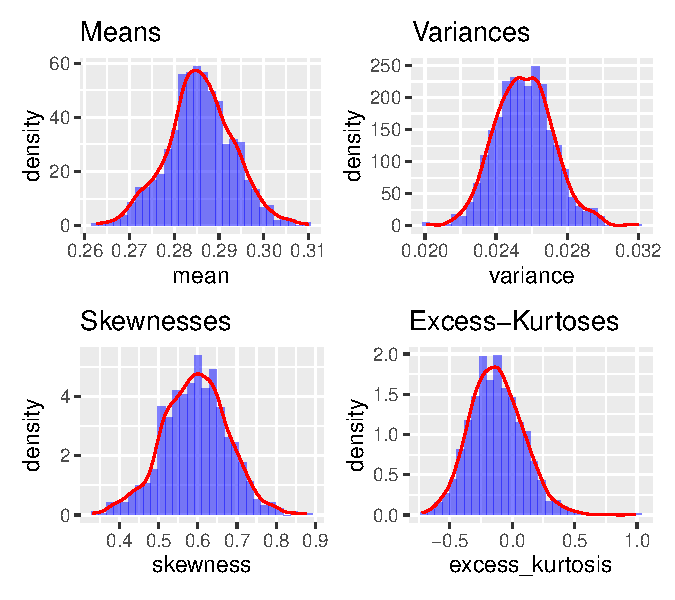
\includegraphics[width=0.435\textwidth]{2x2Plot.pdf}
\newline \newline \indent 
Furthermore, the  \texttt{cumstats} \citep{cumstats} package allowed us to compute the cumulative numerical summaries for each property. For 50 iterations of the alpha = 2 and beta = 5 beta distribution, we ran the \texttt{cumstats} functions on a sample size of 500 to generate a set of 50 line plots for each property. For each property, the plot below shows how with a large enough sample size, all the properties all average out to their true value. Plotted below is another 2x2 grid made using \texttt{patchwork}, however this grid depicts four line graphs, each showing 50 different iterations in which each property averages out to their respective true value as the sample size increases. 
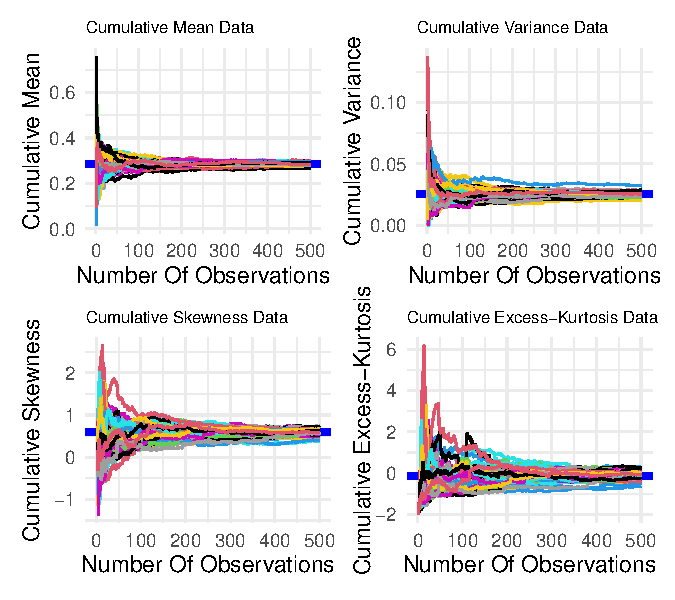
\includegraphics[width=0.435\textwidth]{2x2Grid2.pdf}
\section{Estimators}
In lab 8 we were tasked with computing the Method of Moments (MOM), and Maximum Likelihood (MLE) estimators for the beta distribution which we used to model country death rates worldwide in 2022. The Method of Moments estimator estimates alpha and beta in the beta distribution by equating the sample moments, such as the sample mean and variance, to the theoretical moments of the distribution. The Maximum Likelihood Estimator estimates the parameters of the Beta distribution by maximizing the Beta distribution's likelihood function, which represents the probability of observing the given data as a function of the distribution's parameters.

\section{Example}
Computing the MOM and MLE estimators gave us estimates of the true values for alpha and beta for the beta distribution which can model country death rates worldwide in 2022. The third graph in the appendix shows both the MLE estimator and the MOM estimator superimposed onto the actual data. Although each estimator slightly underestimates the peak of the distribution, they each very closely follow it and are unsurprisingly nearly identical to each other. 

\indent
The final part of lab 8 tasked us with determining which estimator is better in this case, the MOM estimator or MLE estimator. To do this, we set alpha = 8 and beta = 950, estimates determined from when we computed the MOM and MLE estimates. Setting the number of observations for each estimation to 266, we iterated through the MLE and MOM calculations 1000 times, providing us with 1000 method of moments estimates for alpha and beta, and maximum likelihood estimates for alpha and beta. The third graph in the appendix is another 2x2 grid made with \texttt{patchwork} which shows four density curves, each being attributed to either alpha or beta, and either calculated via the MOM estimator or the MLE. Looking at the graphs themselves, it is hard to determine which estimator is better in this case. Each of the alpha plots are nearly indistinguishable from each other, and so are the beta plots.

\indent
To better determine which estimator is more useful for this distribution, we calculated the bias, precision, and mean squared error
for the estimates. The table can be found as the third entry in the appendix. Looking at the table, it becomes apparent that for both alpha and beta, the MOM estimator is slightly more biased, less precise, and has a greater mean squared error. Therefore, in the case of using the beta distribution to model country death rates worldwide in 2022, the MLE estimator is a little bit better at estimating the true values of alpha and beta. This result makes sense because the MLE estimator is typically more consistent with larger sample sizes when compared to the MOM estimator. As a result, the MLE is better suited for providing more reliable estimates of alpha and beta when modeling complex data like country death rates worldwide in 2022.



%%%%%%%%%%%%%%%%%%%%%%%%%%%%%%%%%%%%%%%%%%%%%%%%%%%%%%%%%%%%%%%%%%%%%%%%%%%%%%%%
% Bibliography
%%%%%%%%%%%%%%%%%%%%%%%%%%%%%%%%%%%%%%%%%%%%%%%%%%%%%%%%%%%%%%%%%%%%%%%%%%%%%%%%
\vspace{2em}
\nocite{tidyverse}
\nocite{patchwork}
\nocite{cumstats}

\begin{tiny}
\bibliography{bib.bib}
\end{tiny}
\end{multicols}

%%%%%%%%%%%%%%%%%%%%%%%%%%%%%%%%%%%%%%%%%%%%%%%%%%%%%%%%%%%%%%%%%%%%%%%%%%%%%%%%
% Appendix
%%%%%%%%%%%%%%%%%%%%%%%%%%%%%%%%%%%%%%%%%%%%%%%%%%%%%%%%%%%%%%%%%%%%%%%%%%%%%%%%
\onecolumn
\section{Appendix}

\begin{figure}[!htbp]
    \centering
    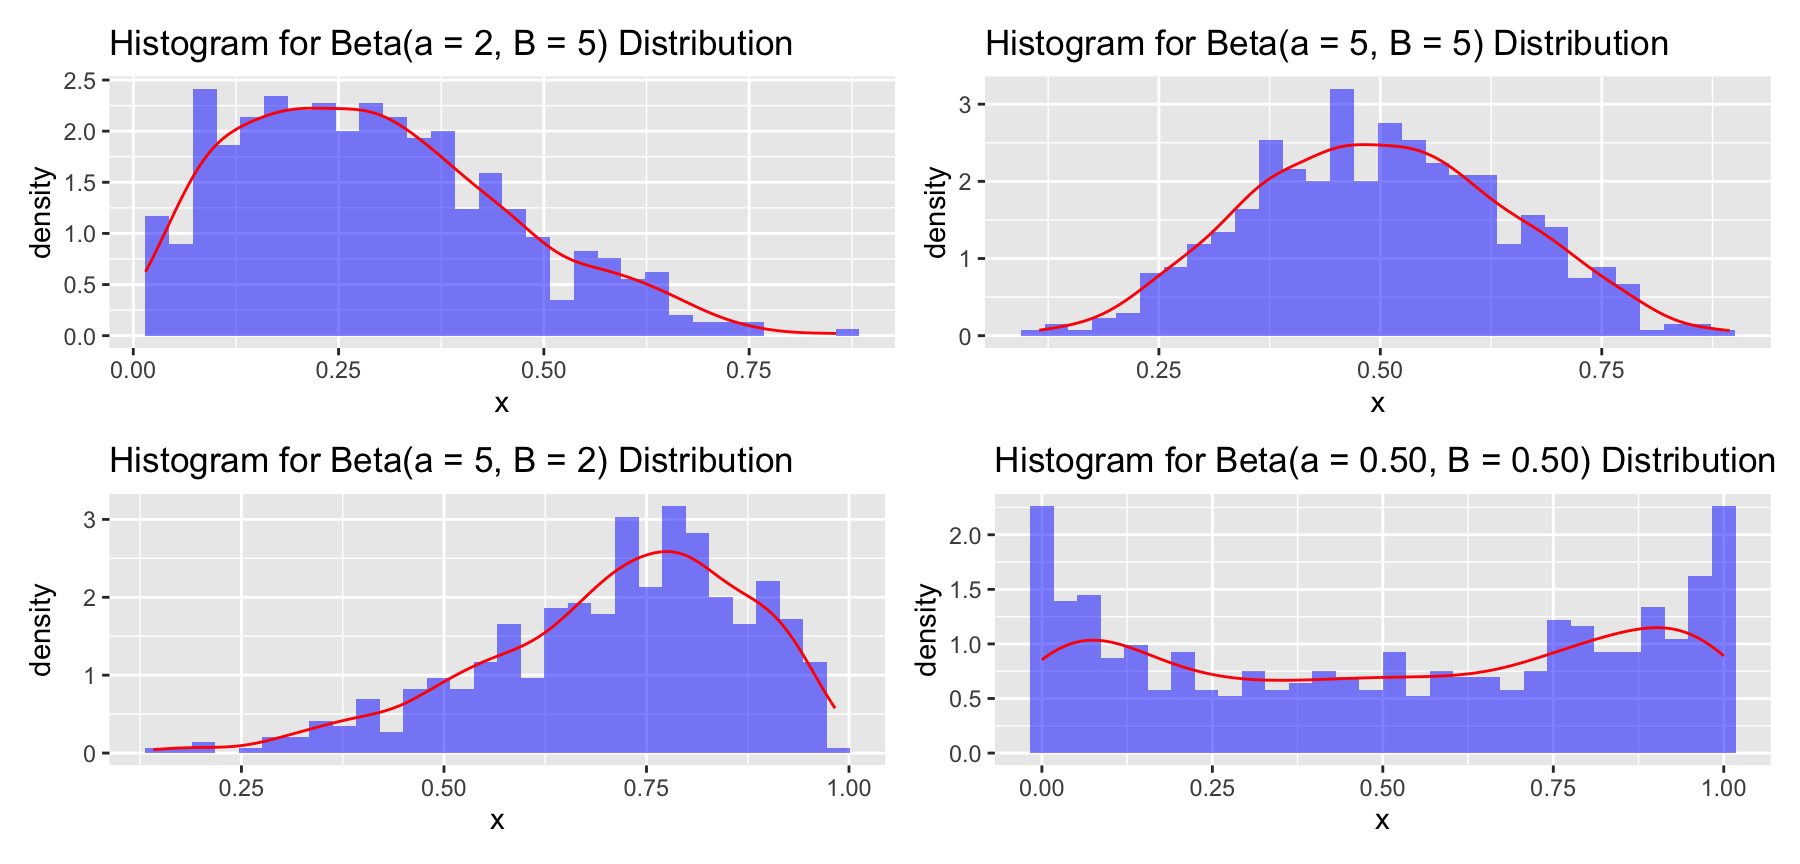
\includegraphics[width=.75\textwidth]{HHHH}
    \caption{}
    \label{fig:first}
\end{figure}

\begin{figure}[!htbp]
    \centering
    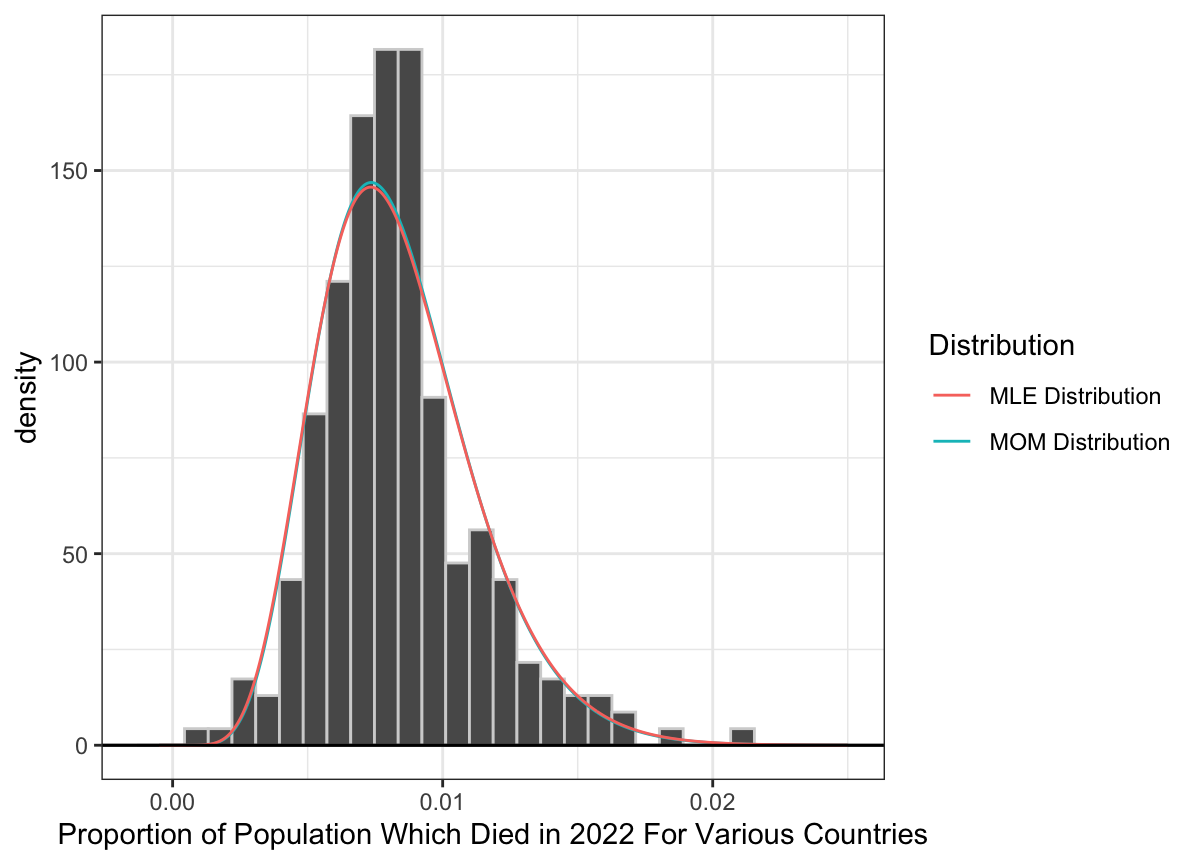
\includegraphics[width=.75\textwidth]{Rplot06.png}
    \caption{}
    \label{fig:second}
\end{figure}

\begin{figure}[!htbp]
    \centering
    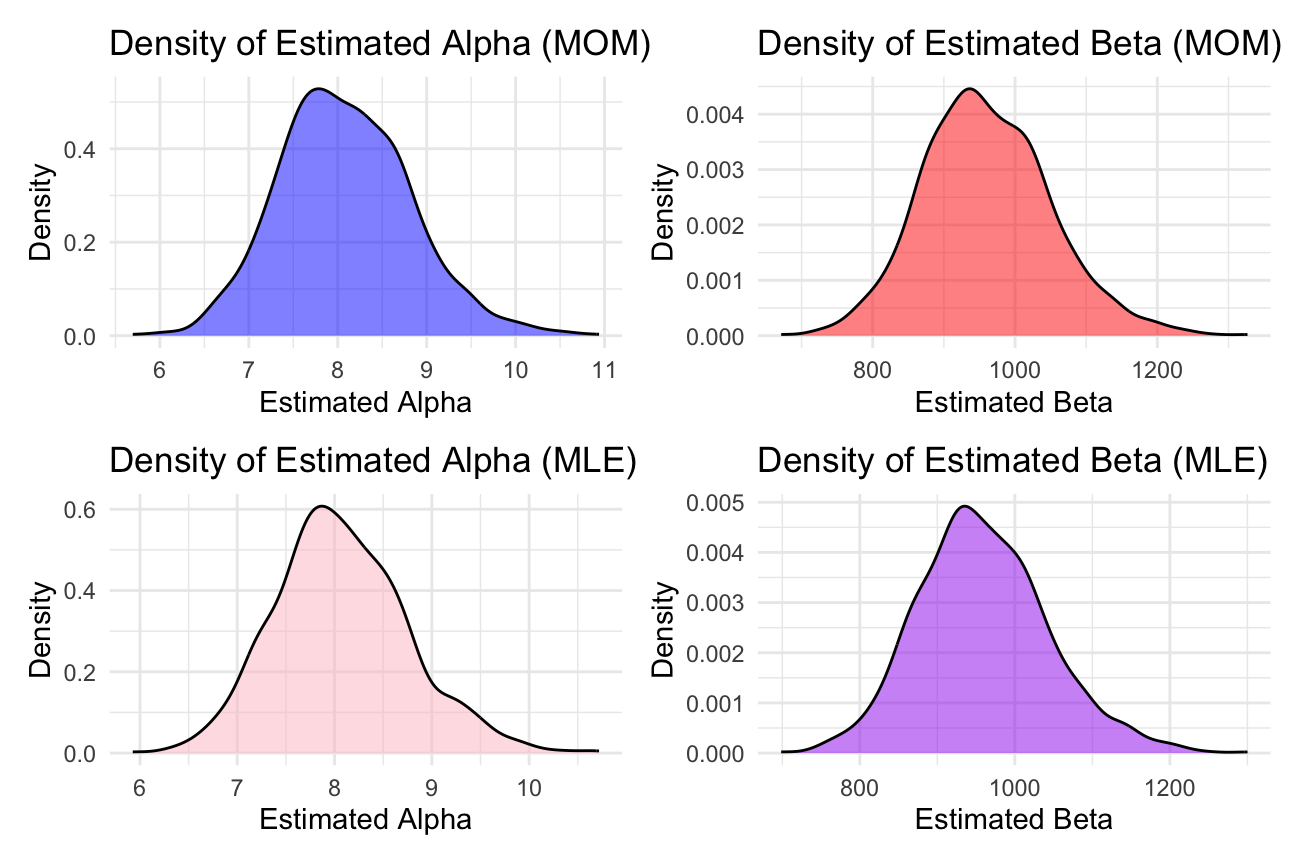
\includegraphics[width=.75\textwidth]{Rplot08.png}
    \caption{}
    \label{fig:third}
\end{figure}

\begin{figure}[!t]
    \vspace{-2in} % Adjust this value to move the figure upwards or downwards
    \centering
    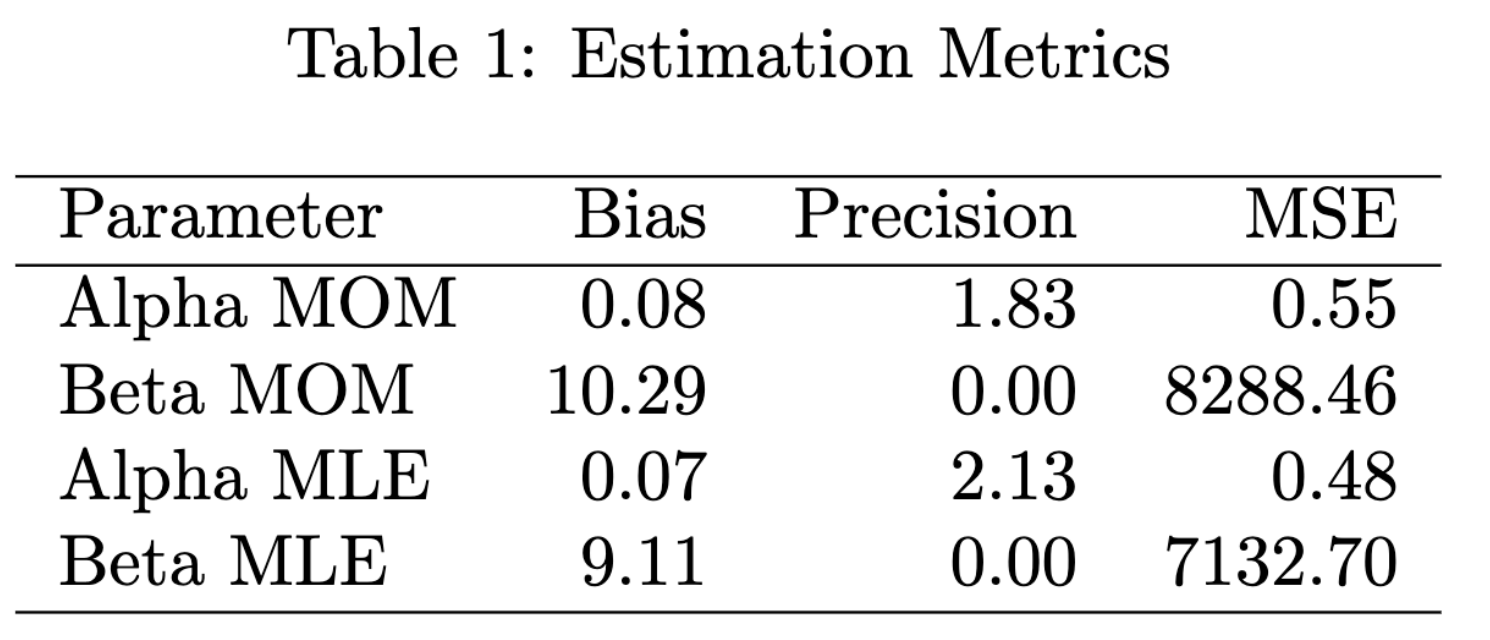
\includegraphics[width=.75\textwidth]{Table}
    \caption{}
    \label{fig:fourth}
\end{figure}




\end{document}
